%%%%%%%%%%%%%%%%%%%%%%%%%%%%%%%%%%%%%%%%%%%%%%%%%%%%%%%%%%%%%%%%%%%%%%%%%%%%%%%
%% Template de Relatório Parcial baseado nas normas da ABNT voltado 
%% para alunos da UEFS, baseado no modelo de TCC
%% Versão 1.3
%% Desenvolvimento: Danilo de Oliveira Gonçalves
%% Adaptação final: João Carlos Nunes Bittencourt
%% Data: 31/03/2011
%% Atualização: 11/08/2011
%
% TODO: Ajustar o espaçamento do cabeçalho do Apêndice e do Anexo.
%%%%%%%%%%%%%%%%%%%%%%%%%%%%%%%%%%%%%%%%%%%%%%%%%%%%%%%%%%%%%%%%%%%%%%%%%%%%%%%
\documentclass{abnt-uefs} % Classe de formatação da UEFS
\usepackage[utf8]{inputenc}
%\usepackage[T1]{fontenc}
\usepackage[call=authordata,alf,abnt-emphasize=bf,abnt-etal-text=emph,abnt-and-type=&,abnt-etal-list=3,abnt-etal-cite=3,recuo=0.0cm]{abntex/abntcite}
\usepackage[brazil]{babel}
\usepackage{mathptmx}
\usepackage[pdftex]{graphicx}
%\usepackage[small,bf]{caption}
\usepackage{longtable}
\usepackage{array}
\usepackage{amssymb,amsmath,amsthm,amsfonts}
%\usepackage{textcomp}
%\usepackage{textcase} 
\usepackage{float} % para as figuras ficarem onde foram colocadas no latex - deve colcoar na figura [H]
\usepackage{color}
%\usepackage{url}
\graphicspath{{figuras/}} % Diretório padrão de figuras.
%%%%%%%%%%%%%%%%%%%%%%%%%%%%%%%%%%%%%%%%%%%%%%%%%%%%%%%%%%%%%%%%%%%%%%%%%%%%%%%
% Este arquivo faz parte do template de Relat�rio Parcial baseado nas normas da ABNT 
%  voltado para alunos da UEFS
% Desenvolvimento: Danilo de Oliveira Gon�alves
% Adapta��o final: Jo�o Carlos Nunes Bittencourt
% Data: 31/03/2011
% Atualiza��o: 30/11/2011
% Descri��o do arquivo:
%   Esse arquivo apresenta as defini��es de constantes que formar�o a capa e 
%   a folha de rosto. Siga as instru��es e modifique de acordo com o que
%   lhe foi orientado.
%%%%%%%%%%%%%%%%%%%%%%%%%%%%%%%%%%%%%%%%%%%%%%%%%%%%%%%%%%%%%%%%%%%%%%%%%%%%%%%

% ---------- Preambulo ----------
\instituicao{Universidade Estadual de Feira de Santana} % nome da instituicao
\departamento{Colegiado de Engenharia de Computa��o} 
\graduacao{Bacharelado em Engenharia de Computa��o} % nome do curso
\curso{Engenharia de Computa��o}

\documento{Trabalho de Conclus�o de Curso} % tipo de documento
\titulacao{Bacharel} % [Bacharel]

\titulo{T�tulo em Portugu�s} % titulo do trabalho em portugues
\subtitulo{Sub-t�tulo, se necess�rio} % caso necess�rio um sub-t�tulo, utilize este campo
\title{Title in English} % titulo do trabalho em ingles

\autor{Nome Completo} % autor do trabalho
\cita{SOBRENOME, Nome} % sobrenome (maiusculas), nome do autor do trabalho

\palavraschave{Palavra-chave 1, Palavra-chave 2, ...} % palavras-chave do trabalho
\keywords{Keyword 1, Keyword 2, ...} % palavras-chave do trabalho em ingles

\comentario{\UEFSdocumentodata\ apresentado ao \UEFSdepartamentodata\ como requisito parcial para obten��o do grau de \UEFStitulacaodata\ no \UEFScursodata\ da \ABNTinstituicaodata.}

\orientador{Nome do Orientador} % nome do orientador do trabalho
%\orientador[Orientadora:]{Nome da Orientadora} % <- no caso de orientadora, usar esta sintaxe
\coorientador{Nome do Co-orientador} % nome do co-orientador do trabalho, caso exista
%\coorientador[Co-orientadora:]{Nome da Co-orientadora} % <- no caso de co-orientadora, usar esta sintaxe

\local{Feira de Santana} % cidade
\data{2011} % ano



 % Elementos da capa
\begin{document}
    \pagestyle{empty}
    \DeclareGraphicsExtensions{.jpg,.pdf,.mps,.png,.bmp,.eps}
    \capa % geração automática da capa
    \folhaderosto % geração automática da folha de rosto
    %%%%%%%%%%%%%%%%%%%%%%%%%%%%%%%%%%%%%%%%%%%%%%%%%%%%%%%%%%%%%%%%%%%%%%%%%%%%%%%
%% Este arquivo faz parte do template de TCC baseado nas normas da ABNT 
%%  voltado para alunos da UEFS
%% Desenvolvimento: Danilo de Oliveira Gon�alves
%% Adapta��o final: Jo�o Carlos Nunes Bittencourt
%% Data: 31/03/2011
%%%%%%%%%%%%%%%%%%%%%%%%%%%%%%%%%%%%%%%%%%%%%%%%%%%%%%%%%%%%%%%%%%%%%%%%%%%%%%%


% dedicat�ria (opcional)
\begin{dedicatoria}
Texto da dedicat�ria.Texto da dedicat�ria.Texto da dedicat�ria.Texto da dedicat�ria.Texto da dedicat�ria.Texto da dedicat�ria.Texto da dedicat�ria.Texto da dedicat�ria.Texto da dedicat�ria.
\end{dedicatoria}

%\vfill

%\begin{flushright}
%\hfill \textit{Dedico esta monografia a minha fam�lia,\\pelo apoio fornecido e aos meus amigos.\\}
%\end{flushright}

%\vspace*{1cm}

%\clearpage 
    %%%%%%%%%%%%%%%%%%%%%%%%%%%%%%%%%%%%%%%%%%%%%%%%%%%%%%%%%%%%%%%%%%%%%%%%%%%%%%%
%% Este arquivo faz parte do template de TCC baseado nas normas da ABNT 
%%  voltado para alunos da UEFS
%% Desenvolvimento: Danilo de Oliveira Gon�alves
%% Adapta��o final: Jo�o Carlos Nunes Bittencourt
%% Data: 31/03/2011
%%%%%%%%%%%%%%%%%%%%%%%%%%%%%%%%%%%%%%%%%%%%%%%%%%%%%%%%%%%%%%%%%%%%%%%%%%%%%%%

% agradecimentos (opcional)
\begin{agradecimentos}
Texto dos agradecimentos.
\end{agradecimentos}
    \begin{resumo}
Escrever um texto que contemple todo o conte�do do trabalho, com espa�amento
1,5, justificado. Conforme as normas NBR 14724:2011 e NBR 6028:2003,da ABNT,
o resumo � elemento obrigat�rio, constitu�do de par�grafo �nico; uma seq��ncia de
frases concisas e objetivas e n�o de uma simples enumera��o de t�picos, n�o
ultrapassando 500 palavras, O resumo deve ressaltar o objetivo, o m�todo, os
resultados e as conclus�es do documento. Deve-se usar o verbo na voz ativa e na
terceira pessoa do singular. Devem ser seguido, logo abaixo, das palavras
representativas do conte�do do trabalho, isto �, palavras-chave e/ou descritores,
que s�o palavras principais do texto, sendo de 3 a 5, separadas por ponto)
\end{resumo}	
    \begin{abstract}
Abstract text (maximum of 500 words).
\end{abstract}

    \listadefiguras % geracao automatica da lista de figuras
    \listadetabelas % geracao automatica da lista de tabelas
    \listadesimbolos % geracao automatica da lista de símbolos
    \listadesiglas % % geracao automatica da lista de siglas
    % sumario
    \sumario % geracao automatica do sumario
    %---------- Primeiro Capitulo ----------
\chapter{Introdu\c{c}\~ao}
O presente documento \'e um exemplo de uso do estilo de formata\c{c}\~ao \LaTeX\ elaborado para atender \`as Normas para Elabora\c{c}\~ao de Trabalhos Acad\^emicos do curso de Engenharia de Computa\c{c}\~ao da UEFS. O estilo de formata\c{c}\~ao {\ttfamily abnt-uefs.sty} tem por base o pacote abn\TeX~-- cuja leitura da documenta\c{c}\~ao \cite{abnTeX2009} \'e fortemente sugerida~-- e o estilo de formata\c{c}\~ao \LaTeX\ proposto pelo Colegiado do Curso de Engenharia de Computa\c{c}\~ao da UEFS.

Para melhor entendimento do uso do estilo de formata\c{c}\~ao {\ttfamily abnt-uefs.cls}, aconselha-se que o potencial usu\'ario analise os comandos existentes no arquivo \TeX\ ({\ttfamily modelo\_*.tex}) e os resultados obtidos no arquivo PDF ({\ttfamily modelo\_*.pdf}) depois do processamento pelo software \LaTeX\ + Bib\TeX~\cite{LaTeX2009,BibTeX2009}. Recomenda-se a consulta ao material de refer\^encia do software para a sua correta utiliza\c{c}\~ao~\cite{Lamport1986,Buerger1989,Kopka2003,Mittelbach2004}.

\textcolor{red}{De 2 e 5 p\'aginas, apresentando a tem\'atica no contexto mais amplo e, em
seguida, chegando ao contexto mais espec\'ifico. Justificar a necessidade/import\^ancia
da pesquisa para o estado da arte e para \'area. Apresentar o objetivo da pesquisa.
Apresentar estrutura da monografia.
}

\section{Motiva\c{c}\~ao}

Uma das principais vantagens do uso do estilo de formata\c{c}\~ao {\ttfamily abnt-uefs.cls} para \LaTeX\ \'e a formata\c{c}\~ao \textit{autom\'atica} dos elementos que comp\~oem um documento acad\^emico, tais como capa, folha de rosto, dedicat\'oria, agradecimentos, resumo, abstract, listas de figuras, tabelas, siglas e s\'imbolos, sum\'ario, cap\'itulos, refer\^encias, etc. Outras grandes vantagens do uso do \LaTeX\ para formata\c{c}\~ao de documentos acad\^emicos dizem respeito \`a facilidade de gerenciamento de refer\^encias cruzadas e bibliogr\'aficas, al\'em da formata\c{c}\~ao~-- inclusive de equa\c{c}\~oes  matem\'aticas~-- correta e esteticamente perfeita.

\section{Objetivos}

\subsection{Objetivo Geral}

Prover um modelo de formata\c{c}\~ao \LaTeX\ que atenda \`as Normas para Elabora\c{c}\~ao de Trabalhos Acad\^emicos da UEFS e \`as Normas de Apresenta\c{c}\~ao de Trabalhos Acad\^emicos do curso de Engenharia de Computa\c{c}\~ao.

\subsection{Objetivos Espec\'ificos}

\begin{itemize}
	\item Obter documentos acad\^emicos automaticamente formatados com corre\c{c}\~ao e perfei\c{c}\~ao est\'etica.
	\item Desonerar autores da tediosa tarefa de formatar documentos acad\^emicos, permitindo sua concentra\c{c}\~ao no conte\'udo do mesmo.
	\item Desonerar orientadores e examinadores da tediosa tarefa de conferir a formata\c{c}\~ao de documentos acad\^emicos, permitindo sua concentra\c{c}\~ao no conte\'udo do mesmo.
\end{itemize}

\subsubsection{Sub-subsection}

    %---------- Segundo Capitulo ----------
\chapter{Desenvolvimento}
\label{chap:desenv}

A seguir ilustra-se a forma de incluir figuras, tabelas, equa\c{c}\~oes, siglas e s\'imbolos no documento, obtendo indexa\c{c}\~ao autom\'atica em suas respectivas listas. A numera\c{c}\~ao sequencial de figuras, tabelas e equa\c{c}\~oes ocorre de modo autom\'atico. Refer\^encias cruzadas s\~ao obtidas atrav\'es dos comandos {\ttfamily \textbackslash label\{\}} e {\ttfamily \textbackslash ref\{\}}. Por exemplo, n\~ao \'e necess\'ario saber que o n\'umero deste cap\'itulo \'e~\ref{chap:desenv} para colocar o seu n\'umero no texto. Isto facilita muito a inser\c{c}\~ao, remo\c{c}\~ao ou reloca\c{c}\~ao de elementos numerados no texto (fato corriqueiro na escrita e corre\c{c}\~ao de um documento acad\^emico) sem a necessidade de renumer\'a-los todos.

\section{Figuras}

Na figura~\ref{fig:dummy} \'e apresentado um exemplo de gr\'afico flutuante. Esta figura aparece automaticamente na lista de figuras. Para uso avan\c{c}ado de gr\'aficos no \LaTeX, recomenda-se a consulta de literatura especializada~\cite{Goossens2007}.

\begin{figure}[!htb]
	\centering
	\caption[Exemplo de uma figura]{Exemplo de uma figura onde aparece uma imagem sem nenhum significado especial.}
	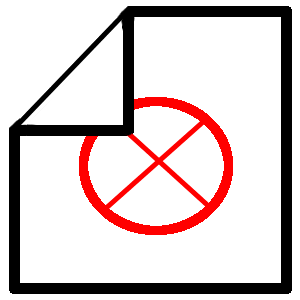
\includegraphics[width=0.2\textwidth]{dummy.png} % <- formatos PNG, JPG e PDF
	\fonte{ABNTEX, 2009\nocite{abnTeX2009}}
	\label{fig:dummy}
\end{figure}

\section{Tabelas}

Tamb\'em \'e apresentado o exemplo da Tabela~\ref{tab:correlacao}, que aparece automaticamente na lista de tabelas. Informa\c{c}\~oes sobre a constru\c{c}\~ao de tabelas no \LaTeX\ podem ser encontradas na literatura especializada~\cite{Lamport1986,Buerger1989,Kopka2003,Mittelbach2004}.

\begin{table}[!htb]
	\centering
	\caption[Exemplo de uma tabela]{Exemplo de uma tabela mostrando a correla\c{c}\~ao entre x e y.}
	\label{tab:correlacao}
	\begin{tabular}{c|c}
		\hline \SPACE
		\textbf{x} & \textbf{y} \\ \hline \SPACE
		1 & 2 \\ \hline \SPACE
		3 & 4 \\ \hline \SPACE
		5 & 6 \\ \hline \SPACE
		7 & 8 \\
		\hline 
	\end{tabular}
	\fonte{Pr\'oprio Autor.}
\end{table}

\section{Equa\c{c}\~oes}

A transformada de Laplace \'e dada na equa\c{c}\~ao~(\ref{eq:laplace}), enquanto a equa\c{c}\~ao~(\ref{eq:dft}) apresenta a formula\c{c}\~ao da transformada discreta de Fourier bidimensional\footnote{Deve-se reparar na formata\c{c}\~ao esteticamente perfeita destas equa\c{c}\~oes!}.

\begin{equation}
X(s) = \int\limits_{t = -\infty}^{\infty} x(t) \, \text{e}^{-st} \, dt
\label{eq:laplace}
\end{equation}

\begin{equation}
F(u, v) = \sum_{m = 0}^{M - 1} \sum_{n = 0}^{N - 1} f(m, n) \exp \left[ -j 2 \pi \left( \frac{u m}{M} + \frac{v n}{N} \right) \right]
\label{eq:dft}
\end{equation}

\section{Siglas e s\'imbolos}

O pacote abn\TeX\ permite ainda a defini\c{c}\~ao de siglas e s\'imbolos com indexa\c{c}\~ao autom\'atica atrav\'es dos comandos {\ttfamily \textbackslash sigla\{\}\{\}} e {\ttfamily \textbackslash simbolo\{\}\{\}}. Por exemplo, o significado das siglas\sigla{CCECOMP}{Colegiado do Curso de Engenharia de Computa\c{c}\~ao},\sigla{DAEComp}{Diret�rio Acad\^emico de Engenharia de Computa\c{c}\~ao} e\sigla{UEFS}{Universidade Estadual de Feira de Santana} aparecem automaticamente na lista de siglas, bem como o significado dos s\'imbolos\simbolo{$\lambda$}{comprimento de onda},\simbolo{$v$}{velocidade} e\simbolo{$f$}{frequ\^encia} aparecem automaticamente na lista de s\'imbolos. Mais detalhes sobre o uso destes e outros comandos do abn\TeX\ s\~ao encontrados na sua documenta\c{c}\~ao espec\'ifica~\cite{abnTeX2009}.
    
\chapter{Fundamentação Teórica}
\label{chap:fundam}

\textcolor{red}{Apresentar estudos que contemple a temática abordada. Respeitar a autoria,
nas citações diretas e indiretas. Evitar parágrafos muito longos. Evitar seções e
subseções muito curtas.}

    
\chapter{Metodologia}
\label{chap:metodo}
\textcolor{red}{Descrever as principais a��es realizadas. � preciso justificar, com base na
literatura, a escolha feita pela metodologia, t�cnicas e instrumentos.}


    \chapter{Resultados}
\label{chap:resul}
Apresentar os resultados da sua pesquisa.
    \chapter{Considerações Finais}
\label{chap:conclusao}
Espera-se que o uso do estilo de formata\c{c}\~ao \LaTeX\ adequado \`as Normas para Elabora\c{c}\~ao de Trabalhos de Conclusão de Curso dos estudantes de Engenharia de Computação, da UEFS ({\ttfamily abnt-uefs.cls}) facilite a escrita de documentos no \^ambito desta institui\c{c}\~ao e aumente a produtividade de seus autores. Para usu\'arios iniciantes em \LaTeX, al\'em da bibliografia especializada j\'a citada, existe ainda uma s\'erie de recursos~\cite{CTAN2009} e fontes de informa\c{c}\~ao~\cite{TeX-Br2009,Wikibooks2009} dispon\'iveis na Internet.

Recomenda-se o editor de textos Kile como ferramenta de composi\c{c}\~ao de documentos em \LaTeX\ para usu\'arios Linux. Para usu\'arios Windows recomenda-se o editor \TeX nicCenter~\cite{TeXnicCenter2009}. O \LaTeX\ normalmente j\'a faz parte da maioria das distribui\c{c}\~oes Linux, mas no sistema operacional Windows \'e necess\'ario instalar o software MiK\TeX~\cite{MiKTeX2009}.

Al\'em disso, recomenda-se o uso de um gerenciador de refer\^encias como o JabRef~\cite{JabRef2009} ou Mendeley~\cite{Mendeley2009} para a cataloga\c{c}\~ao bibliogr\'afica em um arquivo Bib\TeX, de forma a facilitar cita\c{c}\~oes atrav\'es do comando {\ttfamily \textbackslash cite\{\}} e outros comandos correlatos do pacote abn\TeX. A lista de refer\^encias deste documento foi gerada automaticamente pelo software \LaTeX\ + Bib\TeX\ a partir do arquivo {\ttfamily abnt-uefs.bib}, que por sua vez foi composto com o gerenciador de refer\^encias JabRef.

O estilo de formata\c{c}\~ao \LaTeX\ do curso de Engenharia de Computação da UEFS foi elaborados por João Carlos Nunes Bittencourt (joaocarlos@ecomp.uefs.br), e este exemplo de utiliza\c{c}\~ao adaptado de Diogo Rosa Kuiaski (diogo.kuiaski@gmail.com) e Hugo Vieira Neto (hvieir@utfpr.edu.br). Sugest\~oes de melhorias s\~ao bem-vindas.

    % Aqui começa a bibliografia da monografia
    \bibliographystyle{abnt-alf}
    \bibliography{abnt-uefs}
    % Apêndice e Anexos
    \apendice
    %\chapter{Título do Apêndice A}
bla bla bla bla bla bla bla bla bla bla bla bla

bla bla bla bla bla bla bla bla bla bla bla bla

%%%%%%%%%%%%%%%%%%%%%%%%%%%%%%%%%%%%%%%%%%%%%%%%%%%%%%%%%%%%%%%%%%%%%%

\chapter{Título do Apêndice B}
bla bla bla bla bla bla bla bla bla bla bla bla

bla bla bla bla bla bla bla bla bla bla bla bla

    \anexo
    %
\chapter{Título do Anexo A}
\vspace{-3cm}
bla bla bla bla bla bla bla bla bla bla bla bla

bla bla bla bla bla bla bla bla bla bla bla bla

%%%%%%%%%%%%%%%%%%%%%%%%%%%%%%%%%%%%%%%%%%%%%%%%%%%%%%%%%%%%%%%%%%%%%%

\chapter{Título do Anexo B}

bla bla bla bla bla bla bla bla bla bla bla bla

bla bla bla bla bla bla bla bla bla bla bla bla

%%%%%%%%%%%%%%%%%%%%%%%%%%%%%%%%%%%%%%%%%%%%%%%%%%%%%%%%%%%%%%%%%%%%%%

\end{document} 